\chapter{Conclusions and Future Work}\label{ch:conclusions}
\begin{addmargin}[2em]{2em}
This chapter summarizes the thesis and discusses open problems and
future work opportunities.
\end{addmargin}

\section{Discussion and Future Work}
Let us introduce possibilities of future work here. Each chapter
describes the future work specific for a particular area or a problem,
while in this chapter we describe possible future directions from the
perspective of the thesis as a whole.

First, we would like to outline possibilities of combining techniques
and problems from various chapters and sources. Then we will outline general 
directions of research for relational data mining.

\subsection{Pindakaas}
In this subsection we outline possibility to expand TaCLe to work in
the supervised setting. We also propose here a language extension to
handle nested functions and make the system robust to the noise.

If we recap the key features of FlashFill \parencite{flashfill} and of TaCLe
\parencite{tacle}, then we would highlight the following:

\textbf{FlashFill:}
\begin{itemize}
\item String transformation: one of its main capabilities is to
  auto-complete strings in a column 
\item Marked input-output columns: one or more columns are used as
  input and one columns is treated as the output of the string
  transformation function
\item Structured search over programs: internally it searches for a
  program that performs the matching transformation while minimizing
  its complexity
\end{itemize}

\textbf{TaCLe:}
\begin{itemize}
  \item Textual and numeric flat Excel formulae: it is not purely
    textual as FlashFill, but it handles both numbers and strings
  \item Unsupervised: the constraints we find do not have marked
    inputs and outputs
  \item Enumerates all constraints matching the data: TaCle does not
    search for a single solution but find the whole set of formula
    (typically, it outputs its condensed representation)
\end{itemize}

We see that there indeed possibilities for creating a system that
would take best from two worlds: supervised optimal constraint
learning robust under the noise.

\begin{figure}[htb]
 \centering
 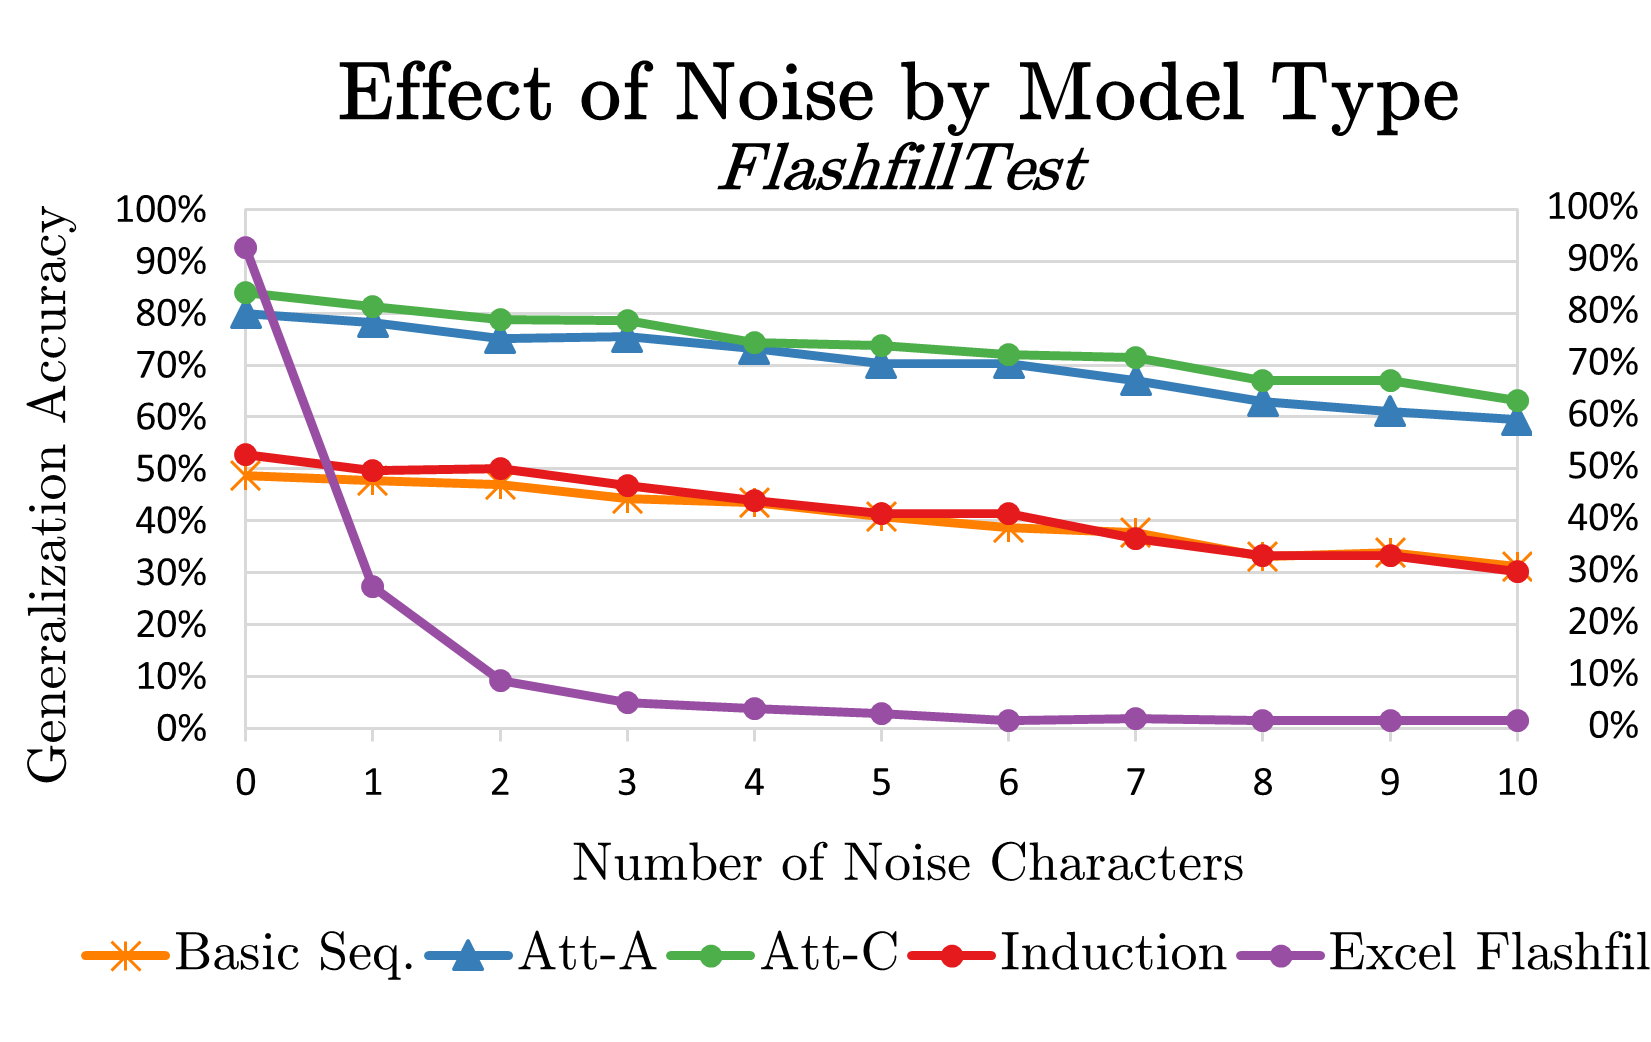
\includegraphics[width=0.7\textwidth]{noise_flashfill.png}
 \caption{We clearly see that FlashFill is highly sensitive to the
   noise (the figure is due to \cite{robustfill})}
  \label{fig:flashfill_noise}
\end{figure}

\begin{figure}[htb]
 \centering
 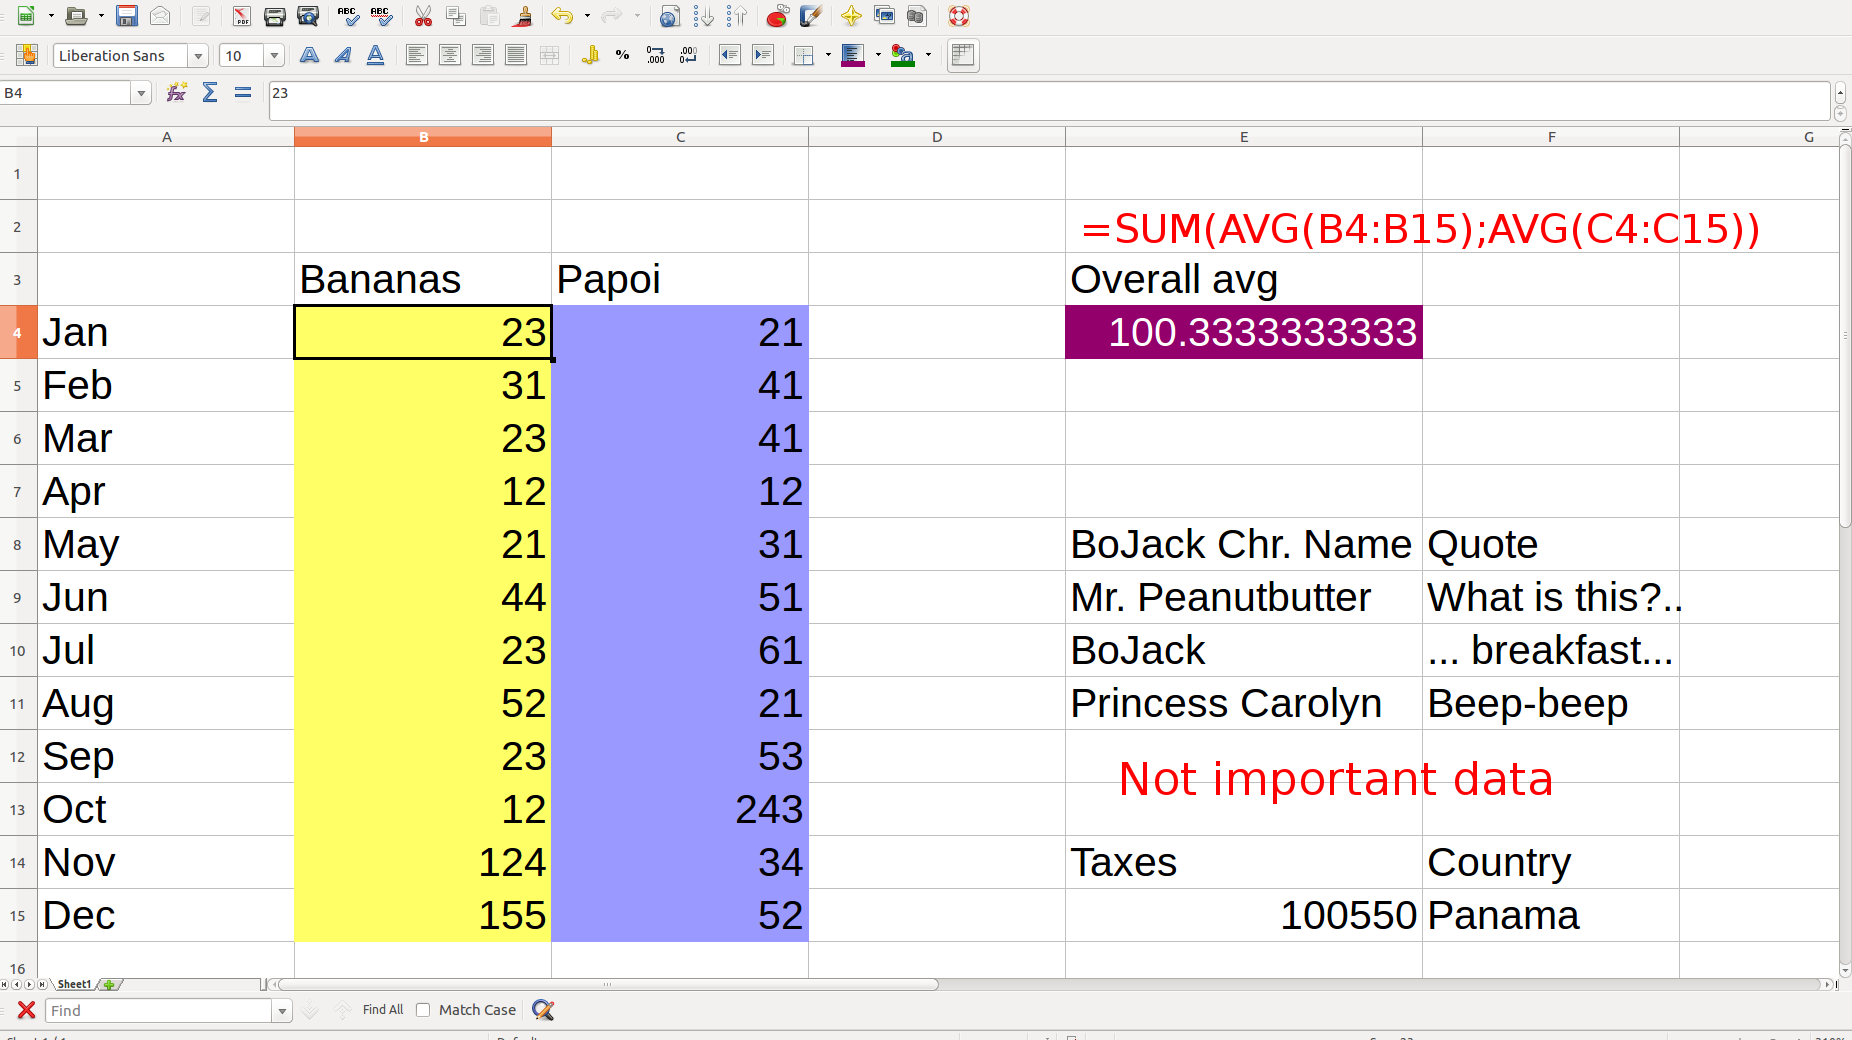
\includegraphics[width=0.7\textwidth]{setting.png}
 \caption{An example of a nested spreadsheet formula}
  \label{fig:nested_formula}
\end{figure}

\begin{figure}[htb]
 \centering
 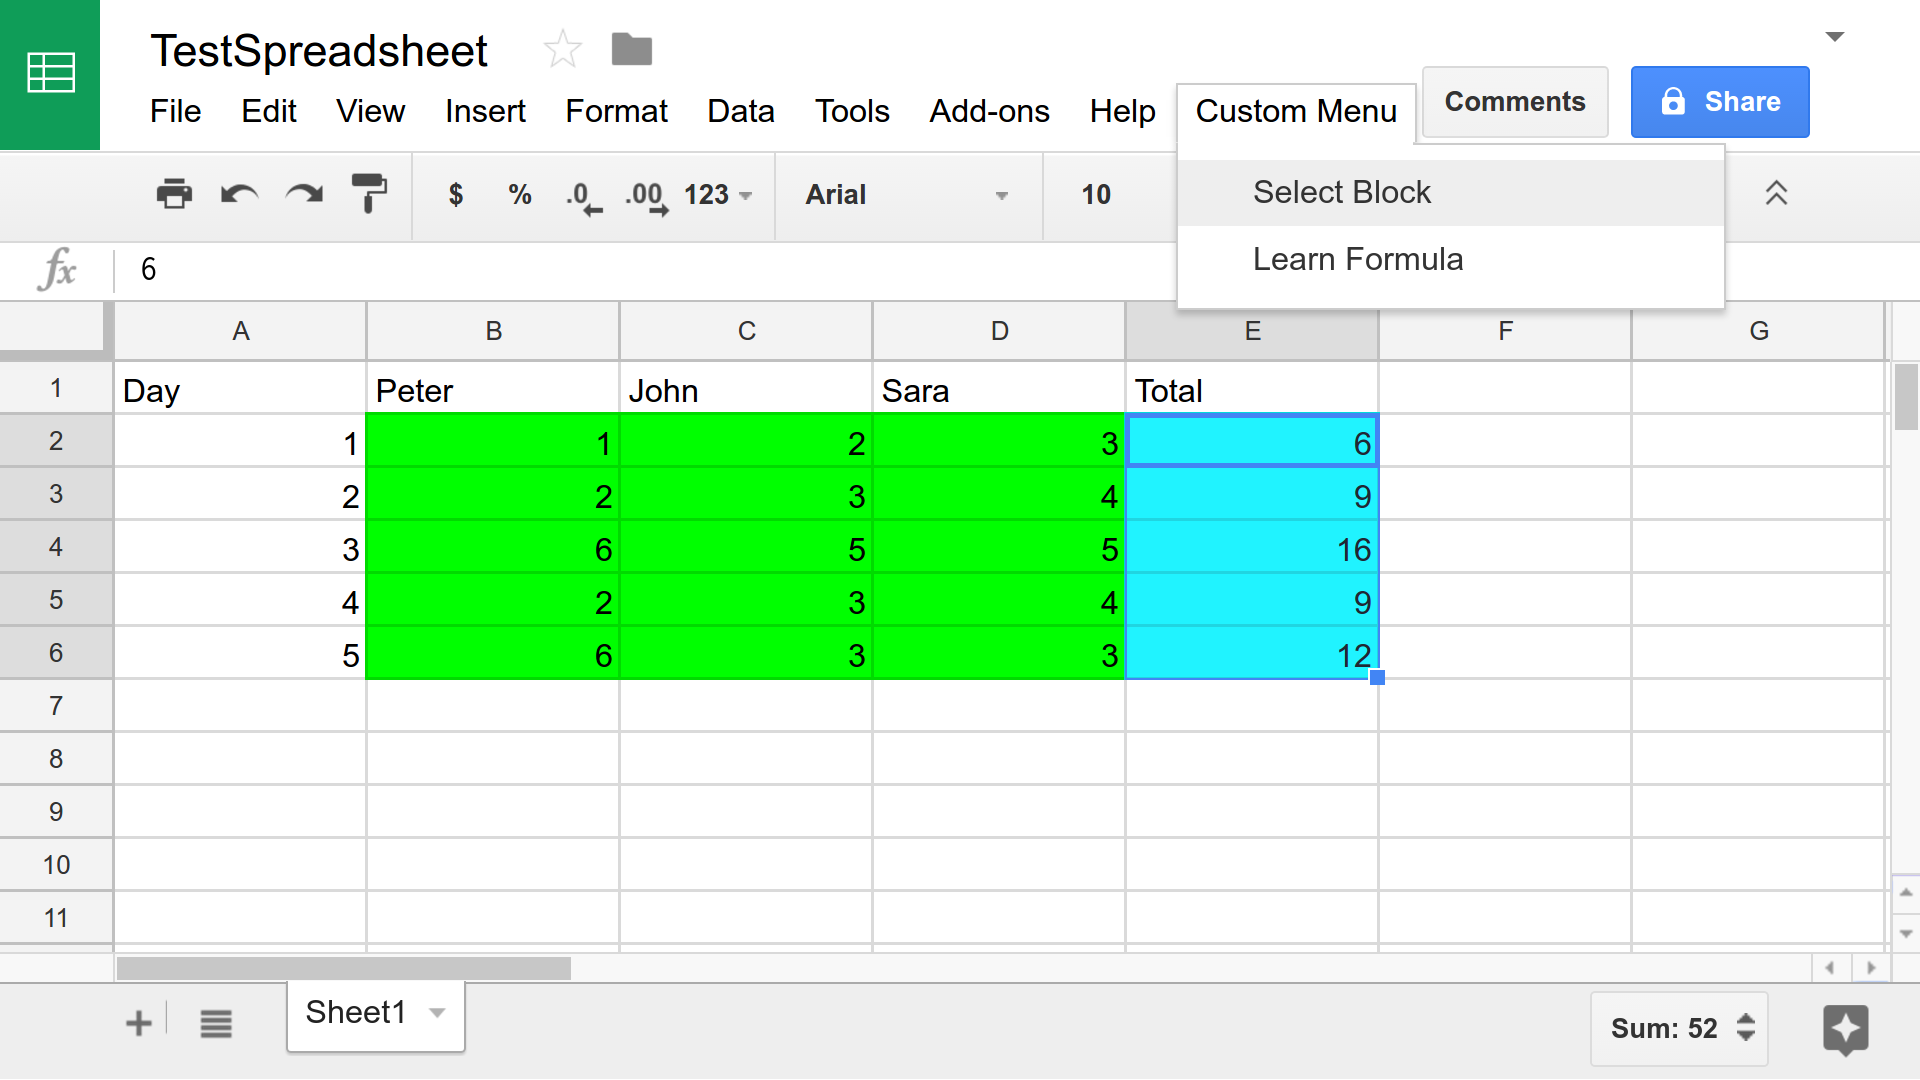
\includegraphics[width=0.7\textwidth]{visualInterface.png}
 \caption{Possible visual interface for Pindakaas}
  \label{fig:visual_interface}
\end{figure}

\textbf{Key Ideas:}
  \begin{itemize}
    \item Use marked or ``supervised'' setting with $\bar x$ for input, $y$ for output
    \item Introduce the loss function $L$ between formula and output
    \item Search for the best fitting formula, i.e., $L(f(\bar x),y)$
    \item Penalize complexity with of a formula, i.e., $\mathcal{C}(f)$ is the measure of complexity
  \end{itemize}

\paragraph{Noise handling} FlashFill is highly sensitive to the noise,
see Figure \ref{fig:flashfill_noise},
and TaCle as well. If we want to make TaCLe robust to the noise, we also need to adapt a
statistical methodology. One way to do it is to introduce a loss
function that would measure how close is the formula to the target
output.

\paragraph{Nested formulae} TaCLe is only able to handle flat
formulae, if we want to extend it to the nested formulae, as for
example in Figure \ref{fig:nested_formula}, we need to
put preference of one formula over another. This can be done by means
of regularizing the formula complexity.

This can be achieved by introducing the following optimization
objective:

  \begin{equation*}
    f^* = \min_{f \in F}{L(f(\bar x),y) + \alpha \mathcal{C}(f)}
  \end{equation*}
  where $\alpha$ is a constant, like in SVM

\paragraph{How can we define complexity}
  \begin{itemize}
     \item for any flat formula $f$, it is a constant
       \begin{equation*}
         \mathcal{C}(f) = c_f 
       \end{equation*}
     \item for any nested formula 
       \begin{equation*}
       \mathcal{C}(f(g(x_1),h(x_2))) = \mathcal{C}(f) + \mathcal{C}(g) + \mathcal{C}(h)
       \end{equation*}
  \end{itemize}
  And the penalization constant $\alpha$ can be learned by cross-validation or set as a parameter

To better position Pindakass, let us contrast it with the features of
TaCLe and FlashFill in Table \ref{tab:pindakaas_features}.
\makesavenoteenv{tabular}
\begin{table}
  \begin{tabularx}{\textwidth}{l | X | X | X }
    \textbf{Property} & \textbf{FlashFill} & \textbf{TaCLe} &
    \textbf{Pindakaas} \\ \hline
    Data type & Text & Numeric and Textual &  Numeric and
    Textual\\\hline
    Learns & String transformation & Set of Flat Excel Formulae
    & Single best nested formula\\\hline
    Supervised & Marked columns + examples & Unsupervised &
    Marked columns \\\hline
    Solving & Structured search & Constraint enumeration &
    Regularized optimization \\\hline
    Satisfaction & Exact & Exact &  Best
    matching\\\hline
    Output & set of values & set of formulae & single
    formula\\ \hline
    Anytime & No & No & Yes
  \end{tabularx}
  \caption{Feature comparison between Pindakaas, TaCLe and FlashFill}
  \label{tab:pindakaas_features}
\end{table}


A possible visual interface is depicted in Figure \ref{fig:visual_interface}.

\subsection{Spreadsheet formula sketching}
In this subsection we investigate a possible combination of TaCLe and
ASP sketching, into \textit{Spreadsheet Formula Sketching (SFS)}.

Let us outline how we see the possible problem definition by
outlining an example.

\textbf{Problem:} a set of partially specified constraints (or formulae, equations), can we complete them given examples?
 
  Specification (for consistency, Excel-like)
  \begin{verbatim}
  B1 := ?F1(A1:A10)
  B2 := B1 ?+ ?F2(B1)
  B3 := if B2 ?= 10, then ?F3(B2)
                     else 42
  \end{verbatim}
  And examples:
  \begin{verbatim}
  positive: B1 = 4; B2 = 2; B3 = 42 
  negative: B1 = 1; B2 = 2; B3 =  3
  \end{verbatim}
  

  Completed specification that is consistent with the examples:
  \begin{Verbatim}[commandchars=\\\{\}]
  B1 := \textbf{SUM}(A1:A10)
  B2 := B1 \textbf{-} \textbf{SQRT}(B1)
  B3 := if B2 \textbf{>} 10, then B2\textbf{^2}
                    else 42
  \end{Verbatim}

This combines ideas from both \acrshort{skasp} and \acrshort{tacle}.
  

\section{Relational Data Mining in Future Years}
It is important to outline not only particular applications developed
or inspiring with this thesis but also to give a perspective on the
development of the overall research direction and the field as a
whole.

As indicated in \ref{ch:StructuredMining}, hybridization of
declarative models is promising and fruitful research direction. It
allows one to combine highly efficient specialized algorithms with
general solvers to create, on the one hand, efficient and scalable
systems; and on the other hand, general system that can handle not
only particular restricted problem but the whole class of pattern
mining problems. Similar to the Dominance Programming for Itemset
Mining \cite{dominanceprogramming} and our hybridization approach structured mining \cite{ruleml_hybrid}, we can foresee creation of 
general mining languages that handle various types of data and
multiple types condensed representations, while demonstrating close to
state-of-art performance. These languages would allow a user to
specify all needed building blocks to generate an executable model
that can find all condensed patterns within reasonable time.

On the relational learning side, inspired by the results of TaCLe
\cite{tacle} and \cite{flashfill}, we envision an intelligent
assistant that can help user by analyzing tabular data in a
spreadsheet and suggest possible cleaning transformations, usage of
Excel-like formulae and data compression. The later idea of data
compression, which can be seen as a form of cleaning, connects to the
ideas of Relational Factorization in Chapter \cite{ch:ReDF}.
Similarly, as indicated in \textit{Spreadsheet Formula Sketching}
paragraph, the assistant can allow the user to specify some of the
formulae or constraints, while leaving certain parts open. Then, the
system can infer possible substitutions from the given tabular data.


\section{Summary and Conclusions}
In the introduction chapter we have identified the key research
questions. Now we are going to review these questions and to analyze the answers provided in this thesis.

\begin{description}
\item[\cone] \textit{What are the challenges and advantages of generalizing
    classic data mining problems, such as the Boolean Matrix
  Factorization problem, into the relation setting?}
\end{description}

As we see in Chapter \ref{ch:ReDF}, the key advantage is the
generality and flexibility of the approach, however, it often comes at
the cost of longer runtimes of the method. There are a number of ways
as has been indicated to handle this problem but it should not come as
a surprise that general methods cannot compete out-of-the-box in the efficiency with
a specialized method devoted to only one particular problem. It is
also clear that specialized methods must be significantly modified in
order to be used in a new setting. Our extensive experimental study
also demonstrates that general relational methods are well-suited for
system prototyping.

\begin{description}
    \item[\ctwo] \textit{How can the constraint learning problem be formulated
   and modelled in the relational setting, where data is
   represented as spreadsheets, i.e., connected relations, and constraints are
   tabular Excel-like formulae?}
\end{description}

As has been shown in Chapter \ref{ch:TaCLe}, the problems related to
spreadsheet data are intrinsically relational, since the data itself
consists of multiple relations together with the dependencies between
them. We have introduced the system called \acrlong{tacle}, based on
classic \acrshort{ilp} ideas, to work in this setting. The systems
enumerates the Excel-like constraints by working on them in the same
manner as clause-learning systems do. It is able to detect the most
popular Excel function in the spreadsheet data as within a table as
well as between multiple tables.

\begin{description}
    \item[\cthree] \textit{Given a relational model, represented as a set of logic
    programming rules, can we mark some parts of it such as atoms,
    operators or constants to be uncertain and reconstruct the model
    using a number of positive and negative examples?}
\end{description}

As we have demonstrated in Chapter \ref{ch:Sketching}, given a
partially complete specification of an ASP program, \acrshort{asp}
can successfully learn relational programs based a few examples
provided. We have extensively analyzed the learned programs and
discovered that on average only few, typically between 2-5, examples needed to
converge to a correct solution. Furthermore, we were able to detect
errors in publicly available encodings, we have contacted the authors
and the models were updated.


\begin{description}
\item[\cfour]  \textit{How can we apply declarative relational mining
    techniques, such as logic programming, to structured frequent pattern mining, such as sequence, graph and query mining?}
\end{description}

As indicated in Chapter \ref{ch:StructuredMining}, we have applied 
logic programming methods to the structured mining problems. As the
result, 
a purely declarative model of graph mining has been created. What we
have discovered is that the systems cannot yet handle this type of
models efficiently. Then, to overcome this issue, we have proposed a hybrid model that
first applies a standard pattern mining algorithm and then uses a
logic programming engine. This has lead to an order of magnitude
efficiency jump and, from the practical point of view, it seems to be
the most fruitful direction of future research in declarative pattern
mining.



%%%%%%%%%%%%%%%%%%%%%%%%%%%%%%%%%%%%%%%%%%%%%%%%%%
% Keep the following \cleardoublepage at the end of this file, 
% otherwise \includeonly includes empty pages.
\cleardoublepage

% vim: tw=70 nocindent expandtab foldmethod=marker foldmarker={{{}{,}{}}}
